\documentclass[pdftex,12pt,a4paper]{report}

\usepackage{a4wide}
\usepackage{setspace}
\onehalfspace

\usepackage{natbib}
\bibliographystyle{agsm}
\renewcommand{\bibsection}{\appendix\chapter{\refname}}

\usepackage{url}
% I'm not completely sure what this does...
% http://tex.stackexchange.com/questions/9445/urls-break-compilation
\renewcommand{\harvardurl}[1]{\textbf{URL:} \url{#1}}

\usepackage[pdftex]{graphicx}
\usepackage{todonotes}

\newcommand{\HRule}{\rule{\linewidth}{0.5mm}}

\begin{document}
\begin{titlepage}
\begin{center}

~
\vspace{3cm}

Submitted for the degree of B.Sc. in Computer Science, 2012\\[0.5cm]

% Title
\HRule \\[0.4cm]

{ \huge \bfseries Augmenting a Monte Carlo Tree Search Agent for Ms Pac-Man with Machine Learning Techniques}\\[0.4cm]

\HRule \\[1.5cm]

\begin{minipage}{0.4\textwidth}
\begin{flushleft} \large
\emph{Author:}\\
Stewart \textsc{MacKenzie-Leigh}\\
200714763
\end{flushleft}
\end{minipage}
\begin{minipage}{0.4\textwidth}
\begin{flushright} \large
\emph{Supervisor:} \\
Dr.~John \textsc{Levine}
\end{flushright}
\end{minipage} \\[2cm]

\end{center}

"Except where explicitly stated all the work in this report, including appendices, is my own and was carried out during my final year. It has not been submitted for assessment in any other context."\\

"I agree to this material being made available in whole or in part to benefit the education of future students." \\[0.5cm]

\begin{flushleft}
Signed: \\[0.5cm]
Date:
\end{flushleft}

\end{titlepage}


\pagenumbering{roman}
\listoftodos
\tableofcontents
\listoffigures
\listoftables

\chapter*{Acknowledgements}

I would like to thank my supervisor Dr John Levine for his guidance throughout this project.  Thank you also to Phil Rogers for his help and support.

Finally I am grateful for the moral support from my friends and family during my studies.

\begin{abstract}

The author and colleagues previously developed an agent for Ms~Pac-Man using Monte Carlo tree search, which runs hundreds of simulated games in order to reach a decision about which move to play, in real time.  During these simulated games, a model of ghost behaviour is used: it was found that when this model happens to match the opponent ghost team, the agent performs well; but when the model and opponent do not match, the agents performance is significantly reduced as its decisions are based on mistaken assumptions.  The aim of this project therefore is to develop a ghost model to use during the simulations that learns by observing the opponent, in order to more accurately model the opponent and improve the score.  The learning algorithm chosen employs neural networks.  Hundreds of games were played to test the effectiveness of the approach with the help of an experiment server, developed for the project, to distribute the games over many machines.  The results show that overall, the learning ghost model decreases performance, but certain cases show a significant improvement, and the learning aspect is demonstrated.  Another important conclusion is that neural networks may not have been the best choice, and the report gives various suggestions for further work.

\end{abstract}


\pagenumbering{arabic}

\chapter{Introduction}
\label{ch:intro}

The game of Ms Pac-Man provides a useful environment for evaluating algorithms for realtime decision-making.  

\chapter{Related work}
\label{ch:related}


\section{The Ms~Pac-Man environment}
The original Pac-Man was an arcade game developed by Toru Iwatani, a Japanese games designer working for Namco Company, in 1980~\citep{Samothrakis2011}.  It became hugely successful due to its wide appeal and a number of spin-offs were created.  One of these was Ms~Pac-Man, which was initially created unofficially before being sold to Midway Games, who distributed Namco games in North America.

The original game features a pizza-shaped protagonist ``Pac-Man'' which the player must direct around a maze consuming ``pills'' and occasionally fruit when it becomes available, whilst avoiding the four ghosts (``Pinky'', ``Inky'', ``Blinky'' and ``Clyde'') which attempt to eat Pac-Man.  If they succeed, Pac-Man loses a life.  There are four ``power pills'' in the maze: if Pac-Man eats one, all the ghosts turn blue and become edible.  Eating as many ghosts as possible in this state confers a significant advantage, as not only is the player rewarded with a number of points upon eating a ghost, the number of points on offer for a ghost doubles with each one eaten.  Starting at 200 for the first ghost, it increases to 400, 800, and 1600 for each consecutive ghost eaten whilst the same power pill is still active.  Thus, the total score available from a power pill is 3050 (50 for the power pill itself, and the sum of the scores mentioned above)---this is in contrast to only 10 points for each regular pill consumed.  Once all the pills in a maze have been cleared, the next level is reached.  Ghosts stay edible for decreasing amounts of time in each subsequent level, making it harder both to score points and to stay alive.

The original Pac-Man featured deterministic ghost behaviour and so it is possible to exploit known patterns of behaviour to learn how to play a given level in such a way that the maximum score for that level is always achieved.  However, Ms~Pac-Man features more sophisticated ghost behaviour which involves a level of non-determinism, making it much more difficult to play.  The other notable difference between the two games is that the latter has four levels instead of just one; there are other minor cosmetic differences such as the renaming of the orange ghost previously known as ``Clyde'' to ``Sue'', and the addition of a red bow and lipstick to the Pac-Man character.

Ms~Pac-Man is now more than thirty years old, a considerable time in the technology arena, and much more sophisticated games exist for the exponentially faster hardware available today; however, it remains useful to artificial intelligence research.  Much work has been done in creating game-playing agents for a wide range of games including chess, checkers, Go, and even Jeopardy, and these agents are often at least as good as human champions.  However, the task environment \todo{Read Russell and Norvig} of Ms~Pac-Man presents several interesting challenges.

Unlike the games mentioned above, the Ms~Pac-Man environment is \emph{dynamic} rather than \emph{static}: whilst in chess the state of the game remains fixed between moves, the state in Ms~Pac-Man is continuously changing, even if the agent is not making any moves.  Additionally, rather than being afforded several minutes to deliberate, the agent must post a move relatively frequently (every 40~ms in the framework mentioned below).  Thus, the environment is also \emph{quasi-continuous} as opposed to being completely \emph{discrete} like board games.

Board games also tend overwhelmingly to be \emph{deterministic}, meaning that the results of a move can be completely and exactly determined by the agent.  In contrast, the Ms~Pac-Man environment is \emph{stochastic}: the ghosts incorporate random behaviour and therefore cannot be completely predicted.  Further complicating the problem of predicting the state of the game after a move is the fact that both Ms~Pac-Man and the ghosts make moves \emph{simultaneously} rather than taking turns as in the majority of board games.

However, the player does have knowledge of the whole game state available to them when making a decision, an attribute shared with traditional board games.  Similarly, all actions available to the player in a given state can be fully known and enumerated.

It can be seen that although Ms~Pac-Man is a seemingly simple, having a trivial objective and few rules, it is perhaps deceptively so, and certain aspects of the task environment greatly increase the complexity of developing an effective agent.  Accordingly, the performance of artificial agents falls somewhat short of the scores achieved by human players.

The usefulness of Ms~Pac-Man to the field of artificial intelligence has previously been recognised and there exists a reasonable amount of research on the subject to date.  This has been encouraged by the creation of various frameworks and competitions to facilitate the development of artificial agents.  The original code is closed source and not designed to run on modern computers, and thus frameworks have had to be written to enable custom agent code to interface with the game.  Various authors~\citep{Lucas2005,Koza1992} have implemented their own simulated versions of the game, sometimes with quite different behaviour to the original game. \citet{Robles2009} also implemented their own version, as well as providing a framework which uses a screen capturing technique to allow the agent to extract information out of the original game running in an emulator.  They demonstrated that their simulator framework and the screen capture framework were roughly equivalent.

It is argued that exact equivalence to the real game is not important however, as the main motivation of such research is not necessarily to write an agent capable of playing the real game well (on its own, a goal of somewhat questionable utility); rather it is to write an agent capable of dealing with the kind of complexities inherent in a game such as Ms~Pac-Man.  As long as the simulated task environment is not significantly different to the real one as described above, the same benefits may be derived from the research.  It is nevertheless important to note that scores obtained by agents under different simulators cannot readily be compared.

The framework used in this work, the aforementioned simulator framework, was developed at the University of Essex~\citep{Robles2009} and used to host various competitions such as at the 2009 IEEE Conference on Computational Intelligence and Games (CIG 2012\footnote{\url{http://geneura.ugr.es/cig2012/}}) and at the IEEE World Congress on Computational Intelligence (WCCI 2012\footnote{\url{http://www.ieee-wcci2012.org/}}).  The framework is written in Java and closely replicates the original game, with a few notable exceptions:

\begin{itemize}
\item Ms~Pac-Man and the ghosts travel at the same speed, unless a power-pill is active, in which case Ms~Pac-Man can move faster than the ghosts.  Unlike the original, Ms~Pac-Man does not slow down when eating pills.
\item In the original, ghosts slow down in the ``tunnels'' at the side of the screen, providing an opportunity to put some distance between Ms~Pac-Man and a pursuing ghost.  This is not the case in the simulator.
\item The simulator does not include the bonus fruit.
\item The behaviour of the ghosts can be determined by any custom ghost controller class.  This is a significant difference which makes the task not only much harder, but arguably much more interesting, as tactics which are effective against one ghost ``team'' may not be effective against another.  The competitions generally feature user-submitted ghost teams as well as Ms~Pac-Man controllers and therefore it is not possible to know in advance what ghost teams the agent should be able to play against.  This point is the main reason behind this paper.
\end{itemize}

\section{Monte Carlo tree search}

\subsection{Background in tree search for games}

Traditional tree search algorithms have been successfully applied to numerous board games such as chess and checkers.  However, these algorithms have been found lacking in some areas, as they can be slow to run and require significant domain knowledge to produce effective agents.  More specifically, the \emph{evaluation function} which evaluates the strength of a particular game state has proven particularly difficult to write for many games.

One such game is Go \footnote{see \url{http://www.gobase.org} for an introduction}.  Chess has an 8~$\times$~8 board, and it is relatively easy to calculate from a given chess position which player has the upper hand by considering aspects such as material count and position.  On the other hand, the Go board (known as the \emph{Goban}) ranges from 9~$\times$~9 for beginners up to as large as 19~$\times$~19, and even experts disagree on the quality of given game states.  The technique of alpha-beta search \todo{cite Russell and Norvig} has proven very powerful for chess players, but the significantly higher branching factor of the game tree given by the larger board and the inability to write an effective \emph{evaluation function} for game states renders the technique of alpha-beta search ineffective for Go~\citep{Gelly2006}.

The Scrabble player \emph{Maven} was one of the first players to make use of simulated game play~\citep{Sheppard2002}.  The merits of different actions are evaluated by playing simulated games for each action, giving an insight into which move will prove to be the better choice as the game develops.  A similar technique has also been used for poker~\citep{Billings2002} and for backgammon~\citep{Tesauro1996}.  However, these players used uniform sampling of available actions or incorporated an unreliable heuristic, leading to much unnecessary simulation.  The UCT (``UCB applied to Trees'') algorithm~\citep{Kocsis2006} was developed in order to more intelligent chose actions to dedicate simulation time to; this effectively developed into the Monte Carlo tree search algorithm.

\subsection{The Monte Carlo tree search algorithm}

\begin{figure}
\label{fig:MCTS}
\missingfigure{MCTS diagram (Chaslot maybe)}
\end{figure}

Monte Carlo tree search (MCTS) is a best-first search technique in which many simulated games are run in order to build a tree of possible game states~\citep{Chaslot2008}.  Each node in the tree represents a game state after taking a given action, represented by the edge from the previous state to the new state.  The algorithm has the following four phases (illustrated in figure \ref{fig:MCTS}):

\textbf{Selection} ~Starting at the root node, the algorithm moves through the search tree by selecting a child of the current node according to some selection policy.  In order to avoid wasting time simulating games for poor moves, the policy must show a preference for choosing moves which have already demonstrated a good reward in previous simulations: this is known as \emph{exploitation}.  On the other hand, the policy must also choose nodes which have been sampled less, so that they may be further investigated: this is known as \emph{exploration}.  This \emph{exploitation versus exploration} dilemma is also seen in multi-armed bandit problems, for which various algorithms exist~\citep{Auer2002}.  The application of this type of algorithm to the selection phase of MCTS is what makes it useful over traditional Monte Carlo methods, as it dramatically decreases the search space.  The UCT algorithm~\citep{Kocsis2006} mentioned above is one of the most commonly-used algorithms for this.

\textbf{Expansion} ~Once a leaf node is reached, it may be expanded.  Expanding a node only once a certain sample count has been reached can produce better results \todo{Expansion threshold citation}.  If the node is expanded, one of its children should be chosen as the new leaf node: this can be a random decision, as the algorithm has no other information.

\textbf{Simulation} ~Also called \textbf{roll-out}, this phase involves running a simulated game from the game state represented by the leaf node arrived at.  In some of the earlier specifications of the algorithm, it was stated that the simulation should be continued until the end of the game~\citep{Chaslot2008}; however, it can also be run until some fixed point in the future, such as after a certain amount of moves.

\textbf{Backpropagation} ~After the simulated game has completed, the tree should be updated with the results.  This may be a simple win/loss ratio, but can be more complex.  For example, an n-player game may backpropagate a score for each player~\citep{Samothrakis2011}.

MCTS has been successfully applied to Go~\citep{Gelly2006} where it significantly improved upon the performance of existing players based on traditional tree search.  This is in part due to the efficient reduction in search space afforded by the UCT algorithm, and also because MCTS does not need an evaluation function.  Instead, random games are played from a game-state until the end of the game, and the score is backpropagated to the node.  MCTS has also been shown to be effective in nondeterministic games and those with imperfect information~\citep{Kocsis2006}.

As Ms Pac-Man has a high branching factor and is non-deterministic, MCTS is suited to the task.

\section{Previous Ms Pac-Man agents}

One of the earliest known studies into Ms~Pac-Man was conducted by \citet{Koza1992}, using genetic programming \todo{Add details from book. D006.31 KOZ}.

\citet{Gallagher2003} created a simplified version of the game containing only regular pills and one ghost.  The agent has two states:

\begin{itemize}
\item The \emph{explore} state: Pac-Man is further than a predefined distance from the ghost.
\item The \emph{retreat} state: Pac-Man is closer than the predefined distance to the ghost.
\end{itemize}

For each of the states, the agent has a set of parameterised probabilistic rules; the parameters are learned using the population-based incremental learning (PBIL) algorithm.  The agent was able to learn the parameters and showed some success, however the authors note that it may be infeasible to scale their approach up to the full game.

\todo[inline]{Finish related work section}

\citet{Me2012} developed an agent using Monte Carlo tree search as part of an ensemble approach.  Prior to making a decision, any number of registered \emph{evaluators} are allowed to run to modify the results of the MCTS algorithm.  For example, a simple evalutor could spot moves in the game tree which eat power pills when there is already one active, and apply penalties to the scores of those nodes.  Thus, short- and long-range planning components augment the mid-range planning provided by the MCTS algorithm.

Although traditional MCTS utilises random playouts, the agent described in the behaviour uses more intelligent agents to control the playout behaviour, as this was found to have better results.  The paper explores two cases: the case where the model of the ghost behaviour used in the playouts matches the actual ghost controller being played against, and the case where the controllers differ.  In the former, three out of the four evaluator configurations considered were found to improve the score by a statistically significant amount, whilst the latter showed a significant improvement for only one evaluator.  Over all, the scores for the accurate model case were in the region of 50,000-60,000, a great deal more than the 10,000-15,000 achieved by the inaccurate model.

Clearly accurate domain knowledge improves the performance of the agent.  If the controller used during the playouts could adapt its behaviour based on observations of the controller being played against, one could reasonably expect the agent performance to steadily improve as the simulation model starts to more closely match the opponent controller.  This is the essence of this project.

\section{Neural networks}

Neural networks are modelled after the nervous system in humans and animals.  This is composed of (in humans, many billions of) cells called \emph{neurons}.  A wide variety of morphologies exist, but the majority of neurons consist of the same three parts: the \emph{dendrites}, highly branched structures which receive chemical signals from other nearby neurons; the \emph{cell body}, which contains the processes necessary for cell function; and the \emph{axon}, containing a ``trigger zone'' which generates electrical signals over the length of the axon if the input to the dendrites reaches a certain threshold.  The axon has \emph{axon terminals} at the opposite end to the dendrites and cell body; these transmit chemical messengers into the dendrites of connected neurons in response to an electrical impulse.  Neurons can be seen as \emph{integrators} as their output is a function of the inputs received from the many connected neurons \cite[p. 152]{Vander}.

Artificial neural networks also consist of large numbers of ``neurons''.  In general, these have a high-dimensional input vector and produce an output which is a non-linear \emph{activation} function (often a sigmoid function) of the input vector and some weights vector \cite[p. 1]{Annema1995}.  It can readily be appreciated how this is analogous to the biological system: the input vector represents the many incoming connections to the dendrites, while the ``trigger zone'' and axon terminals are represented by the activation function and its output.

Each element of the input vector is multiplied by a corresponding element in the weights vector before being summed and used as the input to the activation function; thus, the weights vector controls how much each input affects the output of the neuron.  The weights are adjusted in a \emph{training phase}: by using a large number of training examples where the output expected of the neuron is known, the weights can be iteratively modified according to a learning rule which seeks to minimise the error between the actual output of the neuron and the expected output for each training example \cite[p. 1]{Annema1995}.  This is a form of \emph{supervised learning} \todo{read R and N for supervised learning}.

Although the exact mechanism of learning in the brain is not fully understood, it is thought to operate along similar lines.  In the \emph{long-term potentiation} model, the connections between neurons (called \emph{synapses}) increase in effectiveness when heavily used \cite[p. 271]{Vander}, which is similar in function to the weights which govern the connections between artificial neurons changing value.

\todo[inline]{Add something from Rumelhart et al (D153.4 PAR)}

The type of artificial neural network used in this work is the two-layer feed-forward network \cite[p. 4]{Aleksander1995}.  This consists of a layer of neurons called the \emph{hidden layer}, which computes some internal representation of the inputs \cite[p. 135]{Aleksander1995}, and a connected \emph{output layer}, which computes the final result of the neural network as a function of the output from the hidden layer.  The term "feed-forward" refer to the fact that the input is passed first to the hidden layer, and then fed forward to the output layer.  It has been shown that such a network is capable of approximating any function \cite[p. 10]{Annema1995}.

\todo[inline]{Maybe add Kolmogrov's theorem (p. 10 of Annema) and comment from p. 135 of Aleksander et al}

\subsection{Backpropagation algorithm}

The use of a hidden layer introduces a problem---the expected output for the hidden layer is not known, and so some method must exist for propagating the errors from the output layer in order to train the weights in the hidden layer.  The algorithm used for this purpose in this work is the backpropagation algorithm \cite[p. 134-149]{Aleksander1995}, which will be discussed in more detail in the implementation section.

\chapter{Problem description}
\label{ch:problem}

\section{Overview}

As alluded to in section \ref{sec:previousagents}, when using MCTS for Ms~Pac-Man better final scores are achieved if the ghost controller used during simulated playouts matches the actual opponent controller: the aim of this project is to develop a ghost controller for use during Monte Carlo tree search playouts that is capable of learning its behaviour from observations of the opponent.  This ghost controller developed will be used by the existing MCTS agent developed by \citet{Me2012} for the Ms Pac-Man vs Ghosts framework.

So that the kind of behaviour that the ghost controller will have to learn can be appreciated, there follows in the next section a brief discussion of the sample ghost controllers included in the framework.  Then, the existing agent is explored in some more detail, so that it can be explained how this project will fit into the existing work.  Section \ref{sec:proposedadditions} outlines the requirements for the project and gives an overview of how the problem will be tackled, and finally these requirements are related to the previously-submitted outline specification in section \ref{sec:relationoutlinespec}.


\section{Sample ghost controllers}
\label{sec:sampleghosts}

The Ms~Pac-Man framework used for this project includes several sample ghost controllers.  Although none of them are terribly sophisticated, they provide a basic understanding of the kind of strategies ghost controllers may employ, and are sufficiently different from each other so as to be useful in evaluating the Ms~Pac-Man agent.  They are described briefly below.

\subsection{Legacy}
\label{sec:legacy}
The {\tt Legacy} controller is designed to be passingly similar to the real ghost AI in Ms~Pac-Man.  For three of the ghosts---namely Blinky, Pinky and Inky---the controller returns the next move which takes the ghost closer to Ms~Pac-Man using the path, Euclidian and Manhattan distance measures respectively.  For Sue, the controller returns a random distance.

\subsection{Legacy2TheReckoning}

The behaviour in this controller is the same for all ghosts:

\begin{itemize}
\item If the ghosts are all in close proximity, but not close to Ms~Pac-Man, they are each sent to their own assigned corner of the maze.
\item If a ghost is edible, or Ms~Pac-Man is close to a power pill, the ghost runs away from Ms~Pac-Man.
\item Otherwise, the ghosts' default behaviour is to chase Ms~Pac-Man.
\end{itemize}

It is more difficult to score points against this ghost controller than the previous as the ghosts retreat when edible, making it more difficult to eat them.  It can be seen that even with just this simple rule, if the {\tt Legacy} controller is used during playouts, but the {\tt Legacy2TheReckoning} controller is the actual opponent, the ghosts will be assumed to be travelling in precisely the opposite direction from their actual direction.

The first rule doesn't change the outcome greatly, as the ghosts are generally only next to each other but not next to Ms~Pac-Man when they are exiting the pen.

\subsection{AggressiveGhosts}

Each ghost is instructed to chase Ms. Pac-Man with a certain probability, or execute a random move otherwise.  The framework version has a hard-coded probability of 1.0, so it was rewritten to allow the probability to be supplied in the constructor.

\subsection{RandomGhosts}

All ghosts play random moves with this controller.  Obviously, any attempt to learn a behaviour from this would not be terribly successful.

\subsection{PansyGhosts}

The ghosts in this controller run away from Ms~Pac-Man with a certain probability, and execute a random move otherwise.  Like the {\tt AggressiveGhosts} controller, the probability has been hard-coded to 1.0 in the framework, so the class was rewritten to accept the probability in its constructor.

\subsection{StarterGhosts}

This controller executes the same behaviour for each ghost:

\begin{itemize}
\item If a ghost is edible, or Ms~Pac-Man is next to a power pill, the ghost runs away from Ms~Pac-Man.
\item Failing that, chase Ms~Pac-Man with a certain probability, hard-coded to 0.9 in the framework.
\item Otherwise, chose a random move.
\end{itemize}

This is fairly similar to the {\tt Legacy2TheReckoning} controller, but with the addition of a random element, and without the dispersal tactic.

\section{The existing agent}
\label{sec:existingagent}

The Ms Pac-Man vs Ghosts framework provides the base implementation of the Ms~Pac-Man game: to implement an agent, it is required to subclass the abstract generic class {\tt Controller} and implement the {\tt getMove} function.  The method takes one parameter, the game state, which it can query to make a decision on what move to make.  The return type of the method is specified by the generic type parameter of the class instance:  Pac-Man controllers must extend {\tt Controller{$\langle$}MOVE{$\rangle$}} as they need only return a single move for Ms~Pac-Man, while ghost controllers extend {\tt Controller{$\langle$}EnumMap{$\langle$}GHOST, MOVE{$\rangle\rangle$}}, as they must return a mapping of ghosts to moves.

The framework calls the {\tt getMove} method every 40~ms; if the method takes longer than that time to run, its return value is discarded and the last move returned by the function is selected.  Thus, the method has a strict requirement on running time.

\citet{Me2012} implemented an agent which used Monte Carlo tree search.  It makes use of a class called {\tt MonteCarloPacManSimulator} (henceforth referred to as the simulator class) which runs simulated games and builds a game tree representation using MCTS.  The agent repeatedly calls on the simulator class to run iterations of MCTS while there is still time remaining.  Once near the deadline, no more simulations are performed: if the agent is at a decision point, i.e., a junction, wall or power pill, the best move found by the MCTS is returned; otherwise, the {\tt NEUTRAL} move is returned, instructing the character to continue in the same direction as before.  The tree is only reset if a move is made, allowing the agent to build on the previous simulations each game tick, increasing the deliberation time.

In order to perform the playouts in the MCTS algorithm, the simulator class copies the game state and then repeatedly advances it using particular ghost and Pac-Man controllers until some predefined point (e.g. loss of life, change of level, or after a certain amount of time has elapsed).  The agent was written using a highly modular approach, allowing different implementations to be supplied for various aspects, including the ghost controller to use during playouts.  As discussed in chapter \ref{ch:related}, the final score achieved is an order of magnitude better when the ghost controller used during simulations matches the actual opponent.

\section{Proposed additions to the agent}
\label{sec:proposedadditions}

\begin{figure}
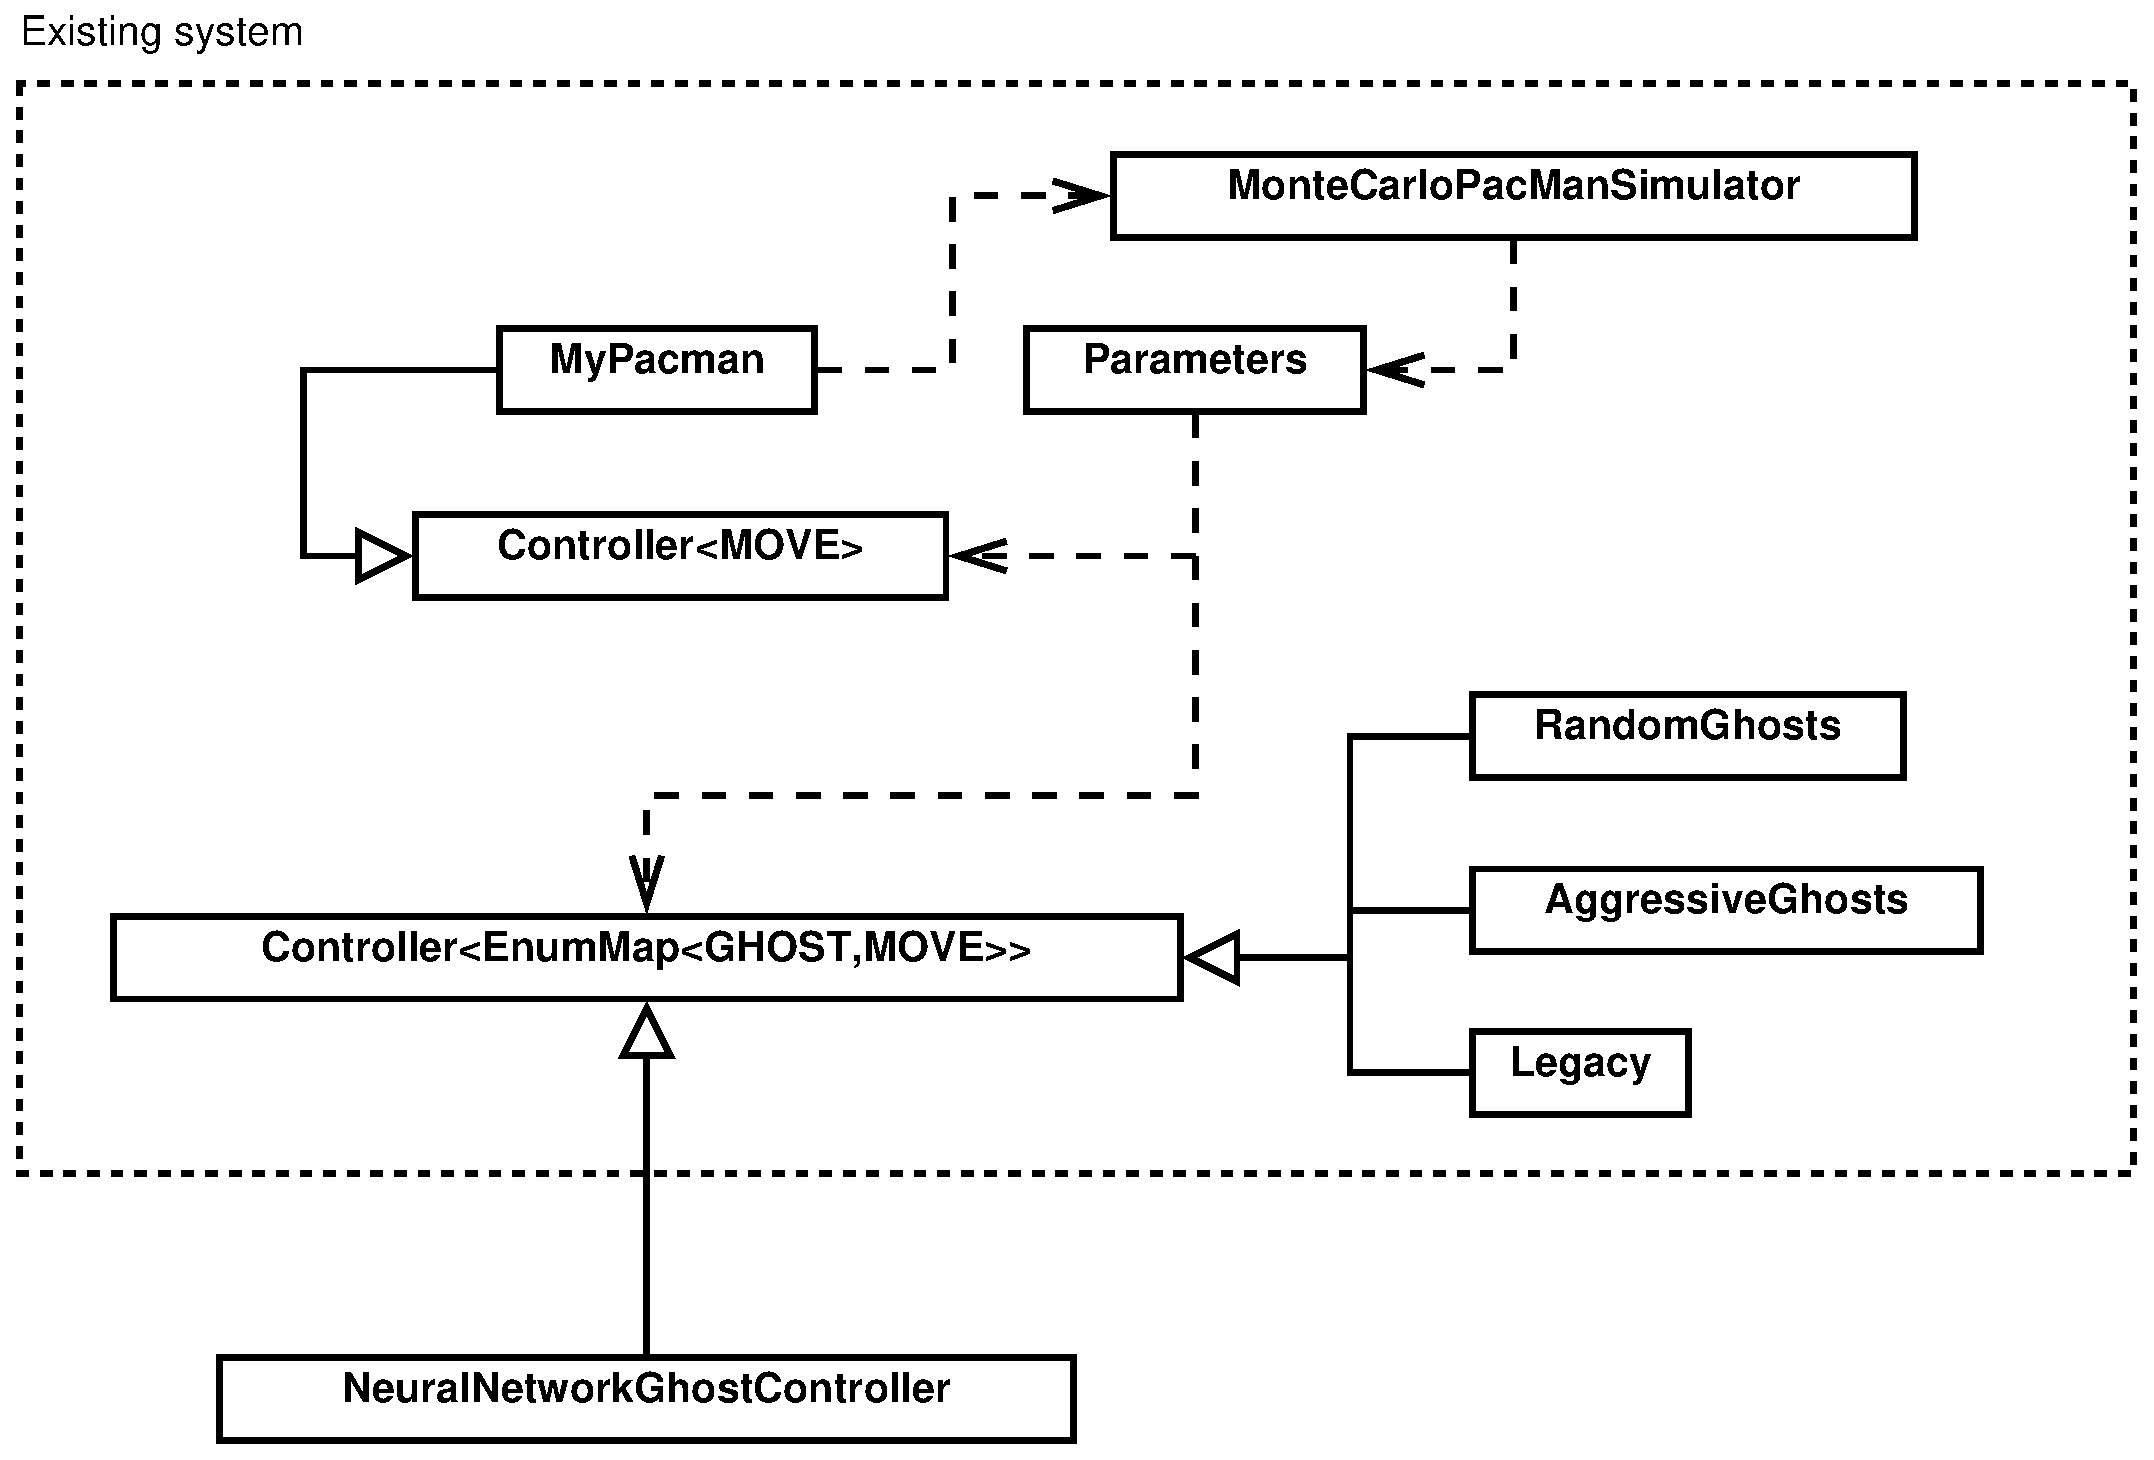
\includegraphics[width=\linewidth]{diagrams/proposed}
\caption[Structural overview]{Structural overview: to implement a Ms Pac-Man agent in the framework, a class extending {\tt Controller<MOVE>} must be created (and it must be called {\tt MyPacman} to be used in the competition).  The existing agent adopts a modular approach: the {\tt Parameters} class contains several fields which specify the behaviour of the algorithm, including one which specifies which ghost controller to use during playouts.  Ghost controllers extend the {\tt Controller<EnumMap<GHOST, MOVE>>} class: some of the example ghost controllers included in the framework are shown.  The proposed addition to the existing agent is a new ghost controller class.}
\label{fig:proposed}
\end{figure}

A neural network is capable of learning arbitrarily complex behaviour from observed examples, so this seemed like a logical avenue of exploration, and is the method chosen for this project.  Each game tick, the game state is recorded; the following tick, it is possible to retrieve the decisions made on that state for each of the ghosts which needed to make a decision.  This input and observed output is used to train the neural network.

During playouts, the ghost controller uses a neural network for each ghost to decide what moves to return: it feeds as input the elements of game state used during training, and feeds this forward through the network.  Since the network has been trained on the observed behaviour of the opponent, the output of the network should in theory approximate the behaviour of the opponent.

The advantage of this approach is that it should be able to approximate the behaviour of a wide variety of agents.  However, neural network algorithms can be expensive to compute---various optimisations are available but these are often very complex.  Obviously, time spent training the neural network is time that could otherwise be spent on MCTS simulations, so a balance must be maintained.  Furthermore, the agent used during the playouts must feed game state data through the neural networks for each ghost to get predicted moves every simulation tick: this is significantly slower than using a random player and further reduces the amount of simulations that can be run.  A further issue is that a ghost only makes 100-200 decisions in a typical game, and this might not be enough data to train the network particularly quickly.

Finally, at the start of the game before the networks have learnt anything, the ghost controller will effectively be random.  This is not a particularly good choice, and the agent may end up losing all its lives before getting a chance to learn anything.  However, a possible solution to this could be feeding the networks with weights learnt offline on an example controller, so that it is producing at least semi-sensible output even at the start of the game.

\section{Requirements}

This discussion draws out a number of requirements.  The addition to the existing agent must perform two functions:

\begin{itemize}
\item Implement a ghost controller which decides on moves player for each ghost, given a game state, using neural networks.
\item Record the decisions of the opponent controller and the game states they were based on each game tick, and use this data to train the neural networks in the ghost controller.
\end{itemize}

Furthermore, the implementation must be fast if it is to be successful.  However, due to the time constraints on the project it may not be possible to implement some of the more advanced algorithms, so a competing requirement is that the implementation must also be reasonably straightforward.

\section{Relation to outline specification}
\label{sec:relationoutlinespec}

Appendix \ref{ap:outlinespec} shows the original outline project specification.  Intially it was decided to write a classification algorithm to classify ghost behaviours into one of several known ghosts, or to attempt to pick values for a parameterised ghost team, and the outline specification is based on this plan.  These techniques are discussed further in section \ref{sec:alternativetreatments} as alternative treatments for the problem, but were dropped in favour of using neural networks.

It was decided near the start of the project that using a classification algorithm would not be as flexible as using neural networks, which had not been investigated much at the time of writing the outline specification.  Although the particular type of machine learning referenced in the outline specification was not used, the aim has remained the same:

``The aim of this project is to investigate using machine learning algorithms to attempt to learn a model of the ghost behaviour in-game, so that the base MCTS algorithm can make more accurate simulations.''

It is worth noting that the original techniques may well yield good results, and they merit further investigation.


\chapter{System design}
\label{ch:design}

\section{Neural network algorithm}
\label{sec:nnalgorithm}
The neural network structure used in the project is a two layer feed-forward neural network \citep[p. 7]{Annema1995}.  The two-layer network features a hidden layer, that is, a layer which is not connected directly to either the input or the output.  It is this feature which gives it the ability to solve ``hard'' learning problems \citep[p. 134]{Aleksander1995}.

However, since the purpose of the hidden layer is to form ``internal representations'' of the data, it is not possible to know what the output of the hidden units should be for a given input.  Therefore, the method of training the network and adjusting the weights of the neurons must be based only on the state of the inputs and outputs to the network, and not of the hidden units \cite[p. 136]{Aleksander1995}.  Backpropagation, discussed in the next section, is one such method of training.

\subsection{Backpropagation}

Much of the theory and the formulae in this section are taken from \citet{Aleksander1995}, chapter 8.  This in turn draws heavily from \citet{Rumelhart1986}, which is much more heavily theoretical and features rigorous proofs of the material presented here; no attempt will be made to replicate this rigour.  Although exactly equivalent, the network here is represented slightly differently and affected formulae are amended accordingly.

\begin{figure}[ht]
\centering
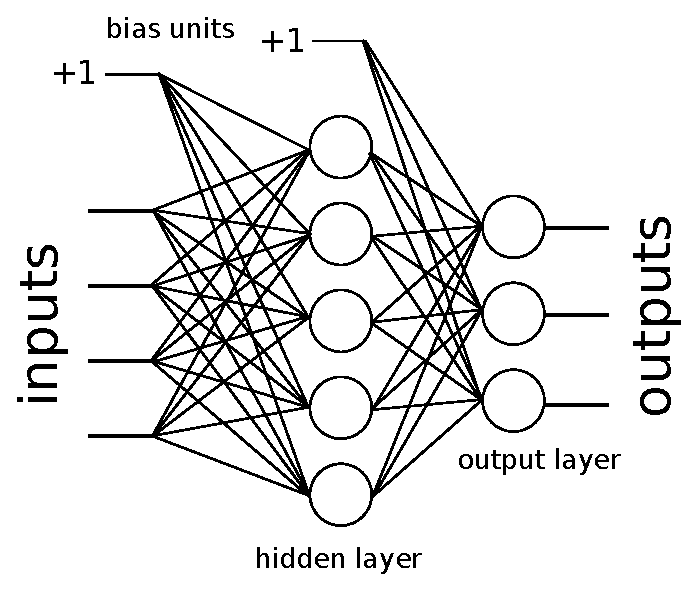
\includegraphics[width=0.5\textwidth]{diagrams/neuralnet}
\caption{A two layer feed-forward neural network}
\label{fig:neuralnet}
\end{figure}

The network topology used is shown in figure \ref{fig:neuralnet}.  It consists of two layers of neurons: the input of every neuron in the first layer (the ``hidden layer'') is connected to every input of the network, and the input of every neuron in the second layer (the ``output layer'') is connected to every output of the first layer.  Finally, the output of the network is defined by the output of the second layer.  The connections between neurons, and betwen inputs and neurons, are each associated with some weight.

Note that some textbooks describe the network as having three layers, the first being the ``input layer'': this description is avoided here, as the inputs are not processed before reaching the hidden layer, i.e., there are no neurons as such in the ``input layer''.

Notice also the two ``bias units'': if the output of each neuron is to compute some aribtrary function of the inputs, they must be able to incorporate some constant value in the function.   \citet{Aleksander1995} describe a \emph{threshold value} which serves the same purpose.  Although a separate threshold value is clearer when dealing with the theory, it will be seen later on that by treating it as a neuron or input which always gives the value 1, the implementation is simplified somewhat.

The \emph{activation} of the $j$th neuron for the $p$th training example, $a_{pj}$, is given by taking the sum for all inputs $i$ multiplied by the corresponding weight, $w_{ji}$.

\begin{equation}
a_{pj} = \sum_{(for~all~i)} w_{ji}o_{pi} + u_j
\label{eq:activation}
\end{equation}

Recalling figure \ref{fig:neuron}, the output $o_{pj}$ of a neuron is the result of some function applied to the activation (equation (\ref{eq:output})).  This function is generally a sigmoid function, and a convenient function to use is shown in equation (\ref{eq:sigmoid}).  It is convenient as its derivative is trivial to determine, and this is required later in the algorithm.  Another popular activation function is $atan(x)$.

\begin{equation}
o_{pj} = f_j(a_{pj})
\label{eq:output}
\end{equation}

\begin{equation}
f(x) = {1 \over 1 + e^{-x}}
\label{eq:sigmoid}
\end{equation}

Using the equations so far, the output of the network can be determined for a given input: first, the outputs of all the neurons in the hidden layer are calculated from the inputs to the neural network; then, the output of the final layer can be calculated from the output of the hidden layer.  It is this process that gives the structure the name ``feed-forward''.

Training the network involves presenting a training example to the network and calculating the output for it using the feed-forward process.  This will give an output, which in the case of a network with no previous training, will be much different from the expected output given by the training data.  The weights are updated as described below to correct for this error, and the training continues.  After many iterations and training examples, the output for a given output will be much closer to the expected value.

Given the $p$th training example, the amount ($\Delta_{p}w_{ji}$) that the weight which joins the $j$th neuron to its $i$th input should be adjusted by is poportional to the calculated error for the unit ($\delta_{pj}$) and a learning rate $\beta$ (equation (\ref{eq:learning})).

\begin{equation}
\Delta_pw_{ji} = \beta\delta_{pj}o_{pi}
\label{eq:learning}
\end{equation}

Calculating the error of output neurons is easy, as the training example states what the expected output is.  The error is therefore the difference between the actual output and the expected output, multiplied by the derivative of the activation function applied to the activation for that neuron (equation (\ref{eq:outputerror})).  Recall the activation function chosen is given by equation (\ref{eq:sigmoid}): its derivative is given by equation (\ref{eq:sigd}).  Note that the value $f(x)$ is the output for the neuron, and has already been calculated by the feed-forward process.

\begin{equation}
\delta_{pj} = (t_{pj} - o_{pj})f'_j(a_{pj})
\label{eq:outputerror}
\end{equation}

\begin{equation}
f'(x) = f(x)\big(1 - f(x)\big)
\label{eq:sigd}
\end{equation}

The errors for the hidden neurons are calculated by propagating the errors back from the output layer, hence the name of the algorithm.  More specifically, the error for the $j$th neuron and the $p$th training example is given by taking the sum of output all errors $k$ multiplied by the corresponding weight $w_{kj}$, all multiplied by the derivative of the activation function applied to the activation for the neuron (equation (\ref{eq:hiddenerror})).

\begin{equation}
\delta_{pj} = \left(\sum_{(for~all~k)}\delta_{pk}w_{kj}\right)f'_{j}(a_{pj})
\label{eq:hiddenerror}
\end{equation}

The described algorithm is a form of gradient descent.  It can be applied to all of the examples in succession, with this being repeated for many iterations; this is called \emph{batch gradient descent}.  As new examples arrive gradually throughout the lifetime of the agent, this project uses the alternative method of \emph{stochastic gradient descent} \citep[p. 720]{RussellNorvig}.

\subsection{Alternatives}

Backpropagation was chosen in this project due to its simplicity and ease of implementation.  Many others have made the same choice, although weaknesses such as slow convergence and a requirement to tune the learning rate are well known.

\citet{Groot1994} showed that algorithms which incorporate higher order information give both a better quality solution (reduced error) and a quicker running time.  By `higher order', the order of the derivatives used by the algorithm is being referred to.  Algorithms which used information from the second derivative of the neural network transfer function were shown to be much more effective.

An exploration of various optimisation algorithms was originally intended as part of this project; however, it turned out to be far too complex to achieve within the time frame.

\section{Proof of concept}

It was necessary to show that it is at least theoretically possible to learn ghost behaviour using neural networks.  First of all, a neural network was implemented in MATLAB; then data from a game was recorded; finally, this data was fed into the neural network implementation to determine if it could be learnt.  The various steps will be described further in the following sections.

\subsection{Vectorised neural network implementation in MATLAB}
\label{sec:matlab}

MATLAB is a mathematical programming language developed by MathWorks.  Although commercial, it is available in many organisations and institutions.  There is also an open source equivalent called Octave: this was initially used, but it lacks several useful functions needed by the project.

One of the benefits of using MATLAB to prototype the neural network is that it can perform operations on variables regardless of whether they represent scalar values or vectors.  For example, in the expression {\tt sin(x)} will return a scalar value if {\tt x} is a scalar, or a matrix of results if {\tt x} is a matrix, using each element in {\tt x} as an input.  Thus, it is convenient if the implementation of the backpropagation algorithm described in section \ref{sec:nnalgorithm} is vectorised.

The inputs to the network are represented as a column vector.  If there are $n$ inputs, there will be $n + 1$ elements in the vector, as the bias unit is added at the top.  If there are $h$ neurons in the hidden layer, the weights which govern the connections between it and the inputs are held in a $h \times (n + 1)$ matrix: for each neuron in the hidden layer, there is a weight to connect it to each of the inputs and the bias unit.  There is a similar matrix for the output layer: in the code, they are called {\tt th1} and {\tt th2} respectively, and they are initially randomly initialised.  This random initialisation is necessary for \emph{symmetery breaking}---if all weight start with the same value, they will always update by the same amount, and the network will be unable to learn anything.

The forward propagation part of the code is given by listing \ref{lst:forward}.  The variable {\tt a1} is the inputs, calculated by taking the $j$th training example and adding the bias unit.  Next {\tt a2}, the hidden layer outputs, is calculated by multiplying the inputs by the weights matrix, applying the activation function\footnote{denoted by the {\tt sig} function, the source code of which is in appendix \ref{ap:matlab}}, and adding the bias unit.  Note that due to the nature of matrix multiplication, the multiply-and-sum operation happens ``for free''.  The output layer is calculated in a similar process, but there is no need to add a bias unit.

\begin{lstlisting}[language=Matlab,label=lst:forward,caption={Forward propagation code},captionpos=b]
a1 = [1; x(j,:)'];
a2 = [1; sig(th1 * a1)];
a3 = sig(th2 * a2);
\end{lstlisting}

After the forward propagation step, backpropagation is performed (listing \ref{lst:backprop}).  The variable {\tt t} represents the target values for the output, and is a vector with a number of elements equal to the number of output nodes.  As described in section \ref{sec:nnalgorithm}, the error of the output nodes ({\tt d3}) is calculated by subtracting the actual output from the target output and multiplying by the derivative of the activation function, defined as {\tt sigd} here.  By using a vectorised implementation, one line of code can perform this function for the whole output layer.

Recall that the error in the hidden layer is given by backpropagating the error from the output layer, using the connecting weights.  The error in the hidden layer is used to calculate the adjustment needed in the weights connecting the hidden layer to the input---since the input is not connected to the bias unit, we do not need to consider it, and that is why the first column (which relates to the bias unit) of {\tt th2} is missed out.

\begin{lstlisting}[language=Matlab,label=lst:backprop,caption={Backpropagation code},captionpos=b]
d3 = (t - a3) .* sigd(a3);
d2 = (th2(:,2:end)' * d3) .* sigd(a2(2:end));
\end{lstlisting}

Now all that remains to be done is to update the weights, shown in listing \ref{lst:update}.  The weights which connect the hidden layer to the input are responsible for any errors resulting in the output of the hidden layer, and the calculated error of the hidden layer is therefore used in updating these weights.  The variable {\tt beta} is the \emph{learning rate}, and governs the rate of gradient descent.  A value of 1 has been found to work adequately.  The weights which govern the connection of the hidden layer and the output layer are updated in a similar fashion.

\begin{lstlisting}[language=Matlab,label=lst:update,caption={Weight update code},captionpos=b]
th1 = th1 + beta * d2 * a1';
th2 = th2 + beta * d3 * a2';
\end{lstlisting}

A full listing of the function described in this section, as well as the listings of the {\tt sig} and {\tt sigd} functions, can be found in appendix \ref{ap:matlab}.  This implementation was verified by ensuring that the network could learn various boolean functions from examples, such as OR, AND, and XOR.  The latter is a `hard' learning problem which can only be learned by multi-layer networks.

\subsection{Logging ghost data}
\label{sec:logging}

In order to prove that the concept was feasible, it was necessary to record the kind of data available in a game to the ghost controller and run the neural network implementation on it to see if it could learn the behaviour.

A class was created, namely {\tt GhostState}, to encapsulate the elements of the game state which matter to a particular ghost.  For example, inside a ghost controller class, the action of a given ghost may be dependent on the ghost's proximity to Ms~Pac-Man; or the next move to make in order to bring the ghost closer to Ms~Pac-Man; or perhaps whether the ghost is edible or not.  This information can be obtained by calling functions on the game state instance passed to the ghost and Ms~Pac-Man controller {\tt getMove} functions (described in section \ref{sec:existingagent}).

A second class, {\tt GhostLogger}, was created to handle recording this ghost information to file. The class holds a reference to an instance of {\tt GhostState} and a {\tt BufferedWriter} which handles writing to the log file.  Every tick, the {\tt log} method on the class is called, which checks if the state information held for the previous tick indicates that the ghost had to make a decision: if it did, then that state information and the decision the ghost made (which is now available, the following tick) is written to the log file as a comma-separated list of floating-point values.  The features are scaled to between 0 and 1 (approximately) by dividing the feature by the the largest value (or a value close to it).  This is necessary to ensure that the network can be trained properly.  Directions (such as the move the ghost took, or the next move away from Ms~Pac-Man) are recorded as four values corresponding to up, down, left and right: a 1 is written in the place for the indicated direction, with the rest being 0.

The ghost the logger is tracking will not make a decision every tick, so a line is only written to the file every few ticks.  Either way, the state the logger holds for the ghost is updated after checking the old state and possibly writing it out.

The {\tt GhostTeamLogger} class was also created to hold references to four instances of {\tt GhostLogger}---one for each ghost---and abstract the details away.  The class implements the {\tt GameTask} interface, which allows it to be added to a list of classes to be invoked each game tick.

The result of running the game with the {\tt GhostTeamLogger} registered as a game task is the creation of four comma-separated variable log files in the log directory, containing the decisions made by each of the four ghosts and the game state data that the decisions were based on.  This data can then be used as training examples for the neural network.

\subsection{Results}
\label{sec:conceptresults}

For each ghost, a neural network was trained using the data in the associated log file, recorded using the methods described in the previous section.  The log files were produced by playing a game against the {\tt Legacy} controller (section \ref{sec:legacy}), and the features chosen to log were fairly arbitrarily chosen as: the level time, the edible score, the number of active power pills, the number of lives remaining for Ms~Pac-Man, the amount of time left for which the ghost will stay edible (or zero if this doesn't apply), the next move away from Ms~Pac-Man and the next move towards Ms~Pac-Man (both using the Manhattan distance measure), and the distance to Ms~Pac-Man from the ghost.  These features were all scaled to be approximately between 0 and 1.  For each of the ghosts Blinky, Pinky, Inky, and Sue, there were 886, 855, 811 and 808 training examples respectively.

After training, each network was used to predict the data it was trained on, and a percentage error rate was obtained.  This was repeated ten times, and averaged for each ghost.  The results are presented in Table \ref{tab:proofconcept}, and give clear indication of learning.  Recall from Section \ref{sec:legacy} that the ghosts in the {\tt Legacy} controller choose the next move towards Ms~Pac-Man using different distance measures: Inky uses the Manhattan measure, which is the one used in the training data, so that could explain why the error rate is zero.  Also, Sue just uses random moves, which would explain why she has the highest error rate.

\begin{table}[ht]
\centering
\begin{tabular}{ll}
\toprule
Ghost & Error rate (\%) \\
\midrule
Blinky & 10.44 \\
Pinky & 24.48 \\
Inky & 0 \\
Sue & 38.61 \\
\bottomrule
\end{tabular}
\caption{Error rates for predicting ghost behaviour}
\label{tab:proofconcept}
\end{table}

Interestingly, although Blinky uses the Path distance measure and Pinky uses Euclidian (which is much closer to the available Manhattan data), it is the former which has the lower error rate.  Even so, that Inky should get a perfect score when supplied with the correct data is cause enough for the investigation in the following section.

Note that the neural networks described above could suffer from \emph{over-fitting}, that is, being particularly good at fitting the training data, but unable to generalise well to new data.  To account for this, the data used as input to the neural network when evaluating the error rate should have been different to the training data.

\subsection{Choosing the neural network features}

The analysis in section \ref{sec:sampleghosts} was the main source of information used when picking the ghost state data to use as input to the neural networks for each ghost (neural network input is often called the \emph{features}).  However, due to the similarity between the Euclidian and Manhattan distance measures, some tests were run to determine if it was really necessary to include both.  The more features a neural network has, the bigger the matrices involved and hence the longer it takes to perform operations with, so it is advantageous to keep the number of features as low as possible.

A game was recorded against the {\tt Legacy} ghost controller in a similar setup to the previous section, except that the next moves towards Ms~Pac-Man were included using all three distance measures.  The networks were then trained using some or all of this data as appropriate in a similar fashion to above.  Note that only the results for Blinky, Pinky and Inky are included, as Sue always returns random moves and bears no relation to the input.

Table \ref{tab:alldm} shows the error rates achieved after training networks for the three ghosts using data which included the next moves towards Ms~Pac-Man using all three distance measures.

\begin{table}[ht]
\centering
\begin{tabular}{ll}
\toprule
Ghost & Error rate (\%) \\
\midrule
Blinky & 7.67 \\
Pinky & 0.39 \\
Inky & 0.13 \\
\midrule
Overall average & 2.73 \\
\bottomrule
\end{tabular}
\caption{Error rates when using all distance measures}
\label{tab:alldm}
\end{table}

The training was repeated for the ghosts using the data from the same game, but with the Manhattan measure removed.  The results (Table \ref{tab:withoutmanhattan}) show the error rate for Inky---the ghost which uses the Manhattan distance measure---increasing from 0.13\% to 7.43\%; however, the overall average does not increase by a great deal.

\begin{table}[ht]
\centering
\begin{tabular}{ll}
\toprule
Ghost & Error rate (\%) \\
\midrule
Blinky & 7.04 \\
Pinky & 0.39 \\
Inky & 7.43 \\
\midrule
Overall average & 4.95 \\
\bottomrule
\end{tabular}
\caption{Error rates when the Manhattan distance measure is unavailable}
\label{tab:withoutmanhattan}
\end{table}

As a result of this, the decision was made to include only the Path and Euclid distance measures.  In the example ghosts, only {\tt Legacy} uses something other than the Path measure, and it is assumed that competition controllers are more likely to mostly only use this measure as well as it is the most useful; the Euclid distance measure is sufficiently similar to make up for the missing Manhattan measure.  At this point, the distance between Ms~Pac-Man and her closest powerpill was also added as a feature.


\subsection{Neural network implementation in Java}

As introduced in section \ref{sec:matlab}, MATLAB makes it possible to perform operations on whole matrices at once.  A method to convert this easily into Java whilst still preserving much of the terseness of the original was sought, and as a result a Matrix class was written to represent matrices in Java\footnote{There are many good matrix libraries for Java, which were considered at the time---however, it was realised that this implementation would have to be heavily optimised for the specific task, which the third-party libraries did not deal with.  See section \ref{sec:efficiency} for more details on the optimisations made.}.  The neural network code using this matrix implementation (listing \ref{lst:javanet}) is appreciably similar the MATLAB implementation, within the constraints of the Java programming language.  This similarity is useful not only as it is easier to programme, but also easier to see that it is correct if it matches the working implementation.

\begin{lstlisting}[language=Java,label=lst:javanet,caption={Java neural network code},captionpos=b]
a1 = Utilities.appendVertical(1, x.part(j, j, 1, -1).transpose());
a2 = Utilities.appendVertical(1, theta1.multiply(a1).apply(sig));
a3 = theta2.multiply(a2).apply(sig);

t = y.part(j, j, 1, -1).transpose();
d3 = t.subtract(a3).elementMultiply(a3.apply(sigd));
d2 = theta2.part(1, -1, 2, -1).transpose().multiply(d3)
        .elementMultiply(a2.part(2, -1, 1, 1).apply(sigd));

theta1 = theta1.add(d2.multiply(a1.transpose()).scale(learningRate));
theta2 = theta2.add(d3.multiply(a2.transpose()).scale(learningRate));
\end{lstlisting}

This implementation was tested with the same test data used in section \ref{sec:conceptresults}, and the algorithm achieved similar results.  It did however run appreciably slower than the MATLAB implementation, a problem addressed in section \ref{sec:efficiency}.

\section{Alternative treatments}
\label{sec:alternativetreatments}
There are various other choices for algorithms to learn the opponent controller behaviour, which are summarised in the following sections.

\subsection{Classifying the ghost behaviour}

One of the first approaches considered at the beginning of this project was to record lots of game data using different opponent ghost controllers, and train a classification algorithm to recognise different kinds of ghost behaviour.  Then during gameplay, the agent could attempt to classify the behaviour observed to determine the known ghost controller which best matches this behaviour, and use this as the controller during playouts.  This has the advantage that a simple classification algorithm, such as logistical regression, is reasonably straightforward to implement.  The downside is that possible opponents in the Ms Pac-Man vs Ghost competitions are extremely diverse, and may not match any of the `known' models.  It would have been interesting to further explore this method if time had available, and it remains a possible opportunity for future work.

\subsection{Reinforcement learning}




\chapter{Implementation details}
\label{ch:implementation}

\section{Structure}

\subsection{Overview}

\subsection{Design patterns}

\section{Matrix efficiency improvements}
\label{sec:efficiency}

\subsection{Na\"{i}ve implementation}

\subsection{An improved representation}

\subsection{Further enhancements}

\chapter{Verification and validation}
\label{ch:verification}

\chapter{Results and evaluation}
\label{ch:results}

\chapter{Summary and conclusions}
\label{ch:summary}

\section{Summary}
An existing agent for Ms~Pac-Man utilising Monte Carlo tree search was augmented by adding a ghost controller to use during MCTS playouts that is capable of learning its behaviour from the opponent ghost team by using neural networks.  In order to evaluate the additions, an ``experiment server'' was created to allow experiments to be specified in JavaScript files and farmed out to many computers to be executed concurrently.

A total of 1900 games were run using the server to investigate the effect of changing various parameters in the algorithm.  The experiment server was a definite success, allowing these games to be run over a few days rather than the week or two it would have otherwise taken.  The success of the learning ghost controller is summarised in the following section.

\section{Conclusions}

As shown in chapter \ref{ch:results}, using the learning controller during playouts instead of a non-learning controller such as {\tt Legacy} appears to decrease the performance of the original agent when averaged over all of the sample ghost controllers in the framework.  However, the framework ghost teams are reasonably similar for the most part, and using the {\tt Legacy} controller during playouts gives reasonable results.

On the other hand, the {\tt PansyGhosts} controller is almost exactly opposite to {\tt Legacy} in that it always runs away from Ms~Pac-Man rather than always running towards her, and using the learning controller during playouts against this team shows a significant improvement in the score over using {\tt Legacy} in the playouts.  It is clear therefore that the controller is able to learn the behaviour of the opponent, which gives an advantage when the opponent is drastically different from {\tt Legacy}.

The results also indicate that the ghost behaviour is particularly easy to learn.  This suggests that neural networks may not have been the best choice, and that some other form of simpler learning would have been better.

\section{Further work}

The performance of the original agent falls short of other current agents using plain Monte Carlo tree search: it would be prudent to investigate the reasons for this and attempt to bring the ``vanilla'' agent to the same level of performance as its contemporaries.

Further investigation is required to understand why the performance of the learning agent is not even as good as the original agent when playing against most of the framework ghosts.  The agent should also be evaluated against better ghost teams as the ones used are very basic and quite similar in most cases.

Finally, using neural networks may not have been the best choice for this project and other machine learning techniques could be investigated.  Section \ref{sec:alternativetreatments} gives several suggestions, such as using a classification algorithm or reinforcement learning.


\bibliography{thesis}

\chapter{Detailed test strategy and test cases}
\label{ch:testing}

\chapter{User guide}
\label{ch:userguide}


\chapter{Program listing}

\end{document}
